% !TeX root = article.tex
\section{Processing plasticity}

In this section, changes to constraint formulation are clarified by doing few simulation steps of rigid and
elastic-plastic examples.

\begin{figure}[htb!]
\centering
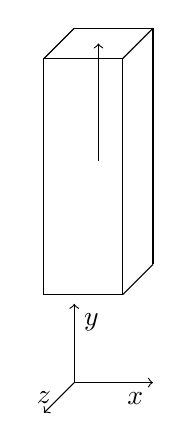
\begin{tikzpicture}
\coordinate (O) at (0,0,0);

% axes
\draw[->] (O) -- (1,0,0) node[anchor=north east]{$x$};
\draw[->] (O) -- (0,1,0) node[anchor=north west]{$y$};
\draw[->] (O) -- (0,0,1) node[anchor=south]{$z$};

% 1,3,1 block, base at y=1.5
\draw (1,1.5,0) -- ++(0,3,0) -- ++(-1,0,0);
\draw (0,1.5,1) -- ++(1,0,0) -- ++(0,3,0) -- ++(-1,0,0) -- ++(0,-3,0);
\draw (1,1.5,0) -- ++(0,0,1);
\draw (0,4.5,0) -- ++(0,0,1);
\draw (1,4.5,0) -- ++(0,0,1);

\draw[->] (0.5,3,0.5) -- ++(0,1.5,0);
\end{tikzpicture}
\caption{Single body model for plasticy processing demonstration.}
\label{fig:tensionModel}
\end{figure}

System has only one dynamic rigid body which is three meters high block of 0.04 \% steel enforced concrete. 
Cross section is one square meter.
Constraint is set so that connecting frame is at top of block. 
In this case frame could be anywhere but if multiple bodies are involved, connecting frame must be defined
so that it reflects wanted scenario.
Concrete density is $2000 \frac{kg}{m^3}$ and steel density id $7800 \frac{kg}{m^3}$. 
Steel is assumed to handle load in elastic-plastic case. Yield stress of steel is 200 MPa.
Gravity is $10 \frac{m}{s^2}$. Simulation step is $\frac{1}{60} s$ and 10 
iterations are done for single step.

Single simulation step is done using following substeps. 
In this work, changes are made only to constraing solving and update actions.
\begin{enumerate}
\item Apply gravity
\item Predict unconstrained motion
\item Predict contacts
\item Perform collision detection
\item Calculate simulation islands(groups). Bodies that are near each other or connected with constraints are grouped in same group.
\item Solve constraints. Both contact and other constraints are processed in this step.
\item Integrate transforms
\item Update actions (callbacks) are called. 
In elastic-plastic case, plasticity is summed and equilibrium point of elastic part is updated if maximum force or moment is exceeded.
\item Activation state of bodies is updated. Bodies that are not active
 are typically marked as sleeping and they are not processed.
\end{enumerate} 

Equation \ref{eq:constraintEquation} is simplified
to \ref{eq:fixedConstraint} in these cases.
\begin{itemize}
\item No rotation takes place. $\omega_1$ and $\omega_2$ are zeros.
\item Constraint force mixing can be ignored.
\item Only vertical velocity is handled.
\item Other involved body is rigid and it does not move.
\end{itemize} 

\begin{equation} \label{eq:fixedConstraint}
m v_y = c 
\end{equation}

Equations \ref{eq:lambdaLow} and \ref{eq:lambdaHigh} are not active for fixed case.
For elastic-plastic case maximum impulse is set to product of yield stress, area of steel enforcement and time step (1330).

Method btSequentialImpulseConstraintSolver::solveGroupCacheFriendlySetup
in \bullet\ was used to pick up values. Actual values for fixed constraint are shown in table
\ref{tab:fixedBlockValues} and values for elastic-plastic case are shown in tables \ref{tab:epBlockValues} and 
 \ref{tab:ep2BlockValues}. There are currently two alternative six-dof-spring constraint implementations in \bullet\ and 
in this work elastic-plastic versions of both of them were developed. 
Constraint activation of older spring and fixed constraints is implemented so that 
they are activated after constraint is violated.
Thus body drops freely during first simulation step and 
gains enough kinetic energy so that higher impulses are needed in few following steps.

\begin{description}
\item[velError] is calculated using velocities and external impulses of connected bodies. 
 In this case, it is dominant contributor for constraint's impulse.
\item[posError] is calculated by constraint. It is significant factor in designing stable constraints.
 \begin{description}
 \item[In fixed case,] value is about 12 times actual position error. Factor 12 is based on time step (60) 
 and default value of error reduction parameter (0.2).
 \item[In elastic plastic case,]  value is set to zero if impulse would be larger than maximum impulse or
spring simulation cannot be done in stable way.
 \end{description}
\item[rhs] is calculated by velError jInv + posError jInv
\item[jInv] is calculated using masses and inertias of connected bodies and constraint geometry. 
In this case, it is mass of body (6000).
\end{description}

\begin {table}[htb!]
\begin{center}
\begin{tabular}{|l| l| l|l|l|l|}
\hline
{\bf Time} & 
{\bf velError} & {\bf posError} & {\bf rhs} &
{\bf velocity} & 
{\bf impulse} \\  \hline
0.017 &  & & & -0.17 & 0 \\  \hline
0.033 &  0.33 & -0.033 & -2200 & 0.033 & 2200 \\  \hline
0.050 &  -0.13 & -0.027 & -960 & 0.027 & 960 \\  \hline
0.067 &  -0.14 & -0.021 & -970 & 0.021 & 970 \\  \hline
0.35... &  -0.17 & $\approx$ 0 & -1000 &0.0 & 1000 \\  \hline
\end {tabular}
\end{center}
\caption {Constraint parameter values for fixed constraint} \label{tab:fixedBlockValues} 
\end {table}


\begin {table}[htb!]
\begin{center}
\begin{tabular}{|l| l| l|l|l|l|l|}
\hline
{\bf Time} & 
{\bf velError} & {\bf posError} & {\bf rhs} &
{\bf velocity} & 
{\bf impulse} & 
{\bf plastic strain} \\  \hline
0.017 &          &    &          & -0.17 & 0 & 0 \\  \hline
0.033 &  -0.33 & 0 & -2000 & -0.11 &  1330 & 0.001 \\  \hline
0.050 &  -0.28 & 0 & -1670 & -0.056 &  1330 & 0.003 \\  \hline
0.067 &  -0.22 & 0 & -1340 &  -0.001&  1330 & 0.004\\  \hline
0.083... &  -0.17 & 0 & -1000 &  0.0&  1000 & 0.004\\  \hline
\end {tabular}
\end{center}
\caption {Constraint parameter values for elastic-plastic constraint} \label{tab:epBlockValues} 
\end {table}

\begin {table}[htb!]
\begin{center}
\begin{tabular}{|l| l| l|l|l|l|l|}
\hline
{\bf Time} & 
{\bf velError} & {\bf posError} & {\bf rhs} &
{\bf velocity} & 
{\bf impulse} & 
{\bf plastic strain} \\  \hline
0.017... & -0.17  & 0 & -1000 & 0       & 1000 & 0 \\  \hline
\end {tabular}
\end{center}
\caption {Constraint parameter values for elastic-plastic constraint 2} \label{tab:ep2BlockValues} 
\end {table}

